\documentclass{beamer}
\usepackage{booktabs}
\usepackage{amsmath}
\usepackage{blkarray}
\usepackage{tikz}

%\usepackage{pdfpages}
%\pdfpagelayout{2 on 1}[letterpaper,border shrink=5mm]

\mode<presentation>
{
%  \usetheme{Malmoe}
\usetheme{default}
%\usecolortheme{seahorse}
  % or ...

 \setbeamercovered{transparent}
  % or whatever (possibly just delete it)
 \setbeamertemplate{footline}[default]
 \setbeamertemplate{navigation symbols}{\insertslidenavigationsymbol\insertframenavigationsymbol\insertdocnavigationsymbol}
}


\usepackage[english]{babel}
% or whatever

%\usepackage[latin1]{inputenc}
% or whatever

%\usepackage{times}
%\usepackage[T1,T5]{fontenc}
% Or whatever. Note that the encoding and the font should match. If T1
% does not look nice, try deleting the line with the fontenc.


\title{Spectral graph theory and its\\
applications to molecular graphs}

%\subtitle{Include Only If Paper Has a Subtitle}

%\author{Dac-Trung Nguyen}
% - Give the names in the same order as the appear in the paper.
% - Use the \inst{?} command only if the authors have different
%   affiliation.

%\institute[NCGC] % (optional, but mostly needed)
%{NIH Chemical Genomics Center\\
%\href{http://www.ncgc.nih.gov}{\texttt{http://www.ncgc.nih.gov}}}
% - Use the \inst command only if there are several affiliations.
% - Keep it simple, no one is interested in your street address.

\date[]% (optional, should be abbreviation of conference name)
{NCATS Informatics Seminar\\ Febuary 17, 2016}
% - Either use conference name or its abbreviation.
% - Not really informative to the audience, more for people (including
%   yourself) who are reading the slides online

%\subject{Theoretical Computer Science}
% This is only inserted into the PDF information catalog. Can be left
% out. 


% If you have a file called "university-logo-filename.xxx", where xxx
% is a graphic format that can be processed by latex or pdflatex,
% resp., then you can add a logo as follows:

\pgfdeclareimage[height=20px]{ncgc-logo}{ncgc_logo}
\logo{\pgfuseimage{ncgc-logo}}



% Delete this, if you do not want the table of contents to pop up at
% the beginning of each subsection:
%\AtBeginSubsection[]
%{
%  \begin{frame}<beamer>
%    \frametitle{Outline}
%    \tableofcontents[currentsection,currentsubsection]
%  \end{frame}
%}


% If you wish to uncover everything in a step-wise fashion, uncomment
% the following command: 

%\beamerdefaultoverlayspecification{<+->}


\begin{document}

\begin{frame}
  \titlepage
\end{frame}

\begin{frame}
  \frametitle{Introduction}
  \begin{itemize}
  \item Spectral graph theory
  \item Well-known matrices
    \begin{itemize}
    \item Adjacency
    \item Laplacian
    \item Normalized Laplacian
    \end{itemize}
  \item Spectral properties
  \item Molecular applications
    \begin{itemize}
    \item Layout
    \item Canonicalization
    \item Invariant
    \item Descriptor
    \end{itemize}
  \item What's next?    
  \item Implementation challenges
  \end{itemize}
\end{frame}

\begin{frame}
  \frametitle{Spectral graph theory}
  \begin{itemize}
  \item Graph $G$ consists of a set of $n$ vertices $V =
    \left\{v_1,v_2,\ldots,v_n\right\}$ and $m$ edges $E =
    \left\{e_1,e_2,\ldots,e_m\right\}$ where  $e_k = v_i\sim v_j$
  \item Let $M$ be a matrix that encodes $G$ based on $V$, $E$, or
    combinations thereof
  \item Spectral graph theory is about understanding the properties
    of $G$ in terms of eigenvalues and eigenvectors of $M$, i.e.,
    \[ M\mathbf{v}_i = \lambda_i\mathbf{v}_i, \]
    where $\lambda_i$ is the $i$th eigenvalue and $\mathbf{v}_i$ is
    the corresponding eigenvector.
  \item The eigenvalues $\{\lambda_i\}$ define the \emph{spectrum} of $G$
  \item Outstanding problem: Which graphs are determined by their
    spectrum?
    \begin{itemize}
      \item Under what conditions do non-isomorphic graphs 
        have the same spectrum?
    \end{itemize}
  \end{itemize}
\end{frame}

\begin{frame}
  \frametitle{Graph spectrum}
  \framesubtitle{Adjacency}
  The adjacency $A$ representation of $G$ is defined as
    \[
    A_{ij}=\begin{cases}
    1 & \quad\text{if } v_i \sim v_j\\
    0 & \quad\text{otherwise}
    \end{cases}
    \]
  \begin{block}{Foundation of H\"uckel theory}
    \emph{The topology of a molecule, rather than its geometry, determines
    the form of the H\"uckel molecular orbitals.}
  \end{block}
  
  \begin{columns}
    \column{1.2 true in}
    \centerline{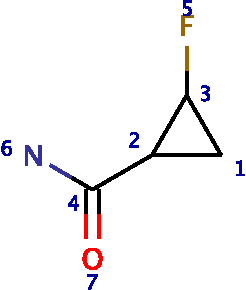
\includegraphics[width=1 true in]{test0-crop}}
    \column{2.8 true in}
    \[
    A = \begin{pmatrix}
0&1&1&0&0&0&0 \\
1&0&1&1&0&0&0 \\
1&1&0&0&1&0&0 \\
0&1&0&0&0&1&1 \\
0&0&1&0&0&0&0 \\
0&0&0&1&0&0&0 \\
0&0&0&1&0&0&0 \\      
    \end{pmatrix}
    \]
  \end{columns}
\end{frame}

\begin{frame}
  \frametitle{Graph spectrum}
  \framesubtitle{Laplacian}
  Let $D$ be the degree matrix of $G$, i.e., $D_{ii} =
  \text{degree}(v_i)$ and 0 elsewhere, we have the Laplacian $L$
  defined as follows
  \[
  L = D - A,
  \]
  where $A$ is the adjacency matrix.
  \begin{columns}
    \column{1.2 true in}
    \centerline{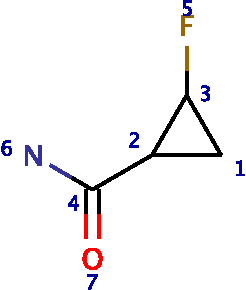
\includegraphics[width=1 true in]{test0-crop}}
    \column{2.8 true in}
    \[
    L = \left(\begin{array}{rrrrrrr}
  2&-1&-1&0&0&0&0 \\
-1&3&-1&-1&0&0&0 \\
-1&-1&3&0&-1&0&0 \\
0&-1&0&3&0&-1&-1 \\
0&0&-1&0&1&0&0 \\
0&0&0&-1&0&1&0 \\
0&0&0&-1&0&0&1 \\
    \end{array}\right)
    \]
  \end{columns}
\end{frame}

\begin{frame}
  \frametitle{Graph spectrum}
  \framesubtitle{Normalized Laplacian}
  The normalized Laplacian is defined as
  \[
  \tilde L = D^{-\frac{1}{2}}LD^{-\frac{1}{2}},
  \]
  or
  \[
  \tilde L_{ij} = \begin{cases}
    1\quad i = j\\
    -\frac{1}{\sqrt{d_id_j}}\quad i \not= j
  \end{cases}
  \]
  where $d_i$ and $d_j$ are the degrees of $v_i$ and $v_j$,
  respectively.
  \begin{columns}
    \column{1.2 true in}
    \centerline{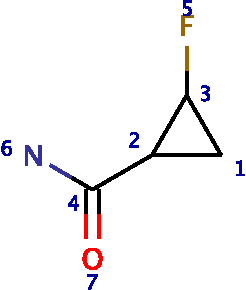
\includegraphics[width=1 true in]{test0-crop}}
    \column{2.8 true in}
    \[
    \tilde L = \tiny\left(\begin{array}{rrrrrrr}
1.0&-0.4&-0.4&0.0&0.0&0.0&0.0 \\
-0.4&1.0&-0.3&-0.3&0.0&0.0&0.0 \\
-0.4&-0.3&1.0&0.0&-0.6&0.0&0.0 \\
0.0&-0.3&0.0&1.0&0.0&-0.6&-0.6 \\
0.0&0.0&-0.6&0.0&1.0&0.0&0.0 \\
0.0&0.0&0.0&-0.6&0.0&1.0&0.0 \\
0.0&0.0&0.0&-0.6&0.0&0.0&1.0 \\      
    \end{array}\right)
    \]
  \end{columns}
\end{frame}

\begin{frame}
  \frametitle{Spectral properties}
  \begin{itemize}
    \item The spectrum of $A$ is bounded by the maximum degree in $G$,
      i.e., $|\lambda_i| \leq \max_k d(v_k)$ for $k = 1, 2, \ldots,
      n$.  For organic molecules, $|\lambda_i| \leq 4$.
    \item $L$ and $\tilde L$'s spectra are non-negative, i.e., $\lambda_i
      \ge 0$. $L$ and $\tilde L$ are semidefinite.
    \item Multiplicity of $\lambda_i = 0$ in $L$ and $\tilde L$ is the
      number of connected components in $G$. 
    \item The spectrum of $\tilde L$ is bounded by 2, i.e., $0 \le
      \lambda_i \le 2$.
    \item Let $\lambda_1 = 0 \le \lambda_2 \le \cdots \le \lambda_n$ for
      $L$ and $\tilde L$. The first non-zero $\lambda_i$ is the
      \emph{algebraic connectivity} index with the corresponding 
      eigenvector known as the \emph{Fiedler} vector. This vector
      provides near-optimal 2-partition of $G$. The Fiedler vector
      is the foundation of many spectral clustering algorithms.
  \end{itemize}
  \begin{columns}
    \column{1 true in}
    \column{1.2 true in}
    \centerline{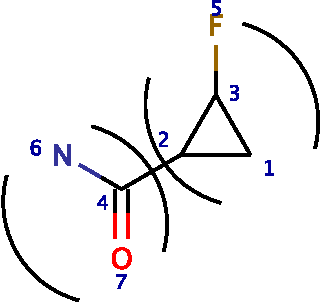
\includegraphics[width=.8 true in]{test0-part-crop}}
    \column{2 true in}
    \[
    \mathbf{v}_2(\tilde L) = \left[\tiny\begin{array}{r}
      0.29255\\
      0.11507\\
      0.44483\\
      -0.53342\\
      0.32870\\
      -0.39416\\
      -0.39416\\
      \end{array}\right]
    \]
    \column{1 true in}
  \end{columns}
\end{frame}

\begin{frame}
  \frametitle{Molecular applications}
  \begin{itemize}
    \item Layout --- for high symmetry graphs, the eigenvectors
      $\mathbf{v}_2$ and $\mathbf{v}_3$ of $L$ can be used as
      coordinates for 2-D embedding.
    \item\textcolor{orange}{Canonicalization --- a simple algorithm
      can be derived based on the eigenvectors of $L$ or $\tilde
      L$. Start with the Fiedler vector and recursively partition the
      vertices until each partition contains only one vertex. The
      canonical ordering is the depth first traversal of the binary
      partition tree.}
  \end{itemize}

  \vskip6em
  \begin{columns}
    \column{2.5 true in}
    \begin{block}{}
      \tiny
      \begin{tikzpicture}
        %\tikzstyle{every node}=[draw,shape=circle];
        \tikz [level 1/.style={sibling distance=15em},
          level 2/.style={sibling distance=10em}, level distance=5em]
        \node {$\mathbf{v}_2$}
        child {
          node {$\{v_1,v_2,v_3,v_5\}$ }
          child {
            node { $\{v_1,v_2,v_3\}$ }
          }
          child {
            node { $\{v_5\}$}
          }
        }
        child {
          node { $\{v_4,v_7,v_6\}$ }
          child {
            node { $\{v_4,v_7\}$ }
          }
          child {
            node { $\{v_6\}$ }
          }
        };
      \end{tikzpicture}
    \end{block}
    \column{3 true in}
  \end{columns}
\end{frame}

\begin{frame}
  \frametitle{Molecular applications (cont'd)}
  \textcolor{orange}{Invariant --- which graphs are determined
    by their spectrum?}
  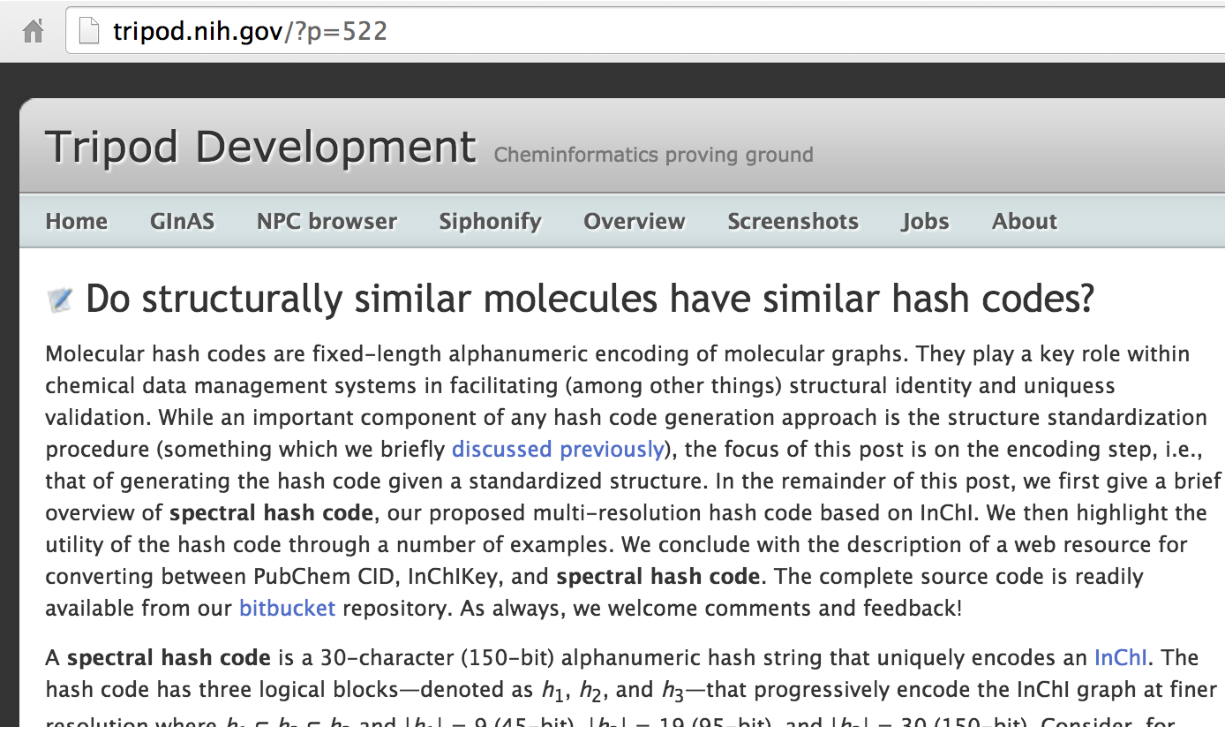
\includegraphics[width=4 true in]{p522-crop}
\end{frame}

\begin{frame}
  \frametitle{Molecular applications (cont'd)}
  \begin{itemize}
    \item \textcolor{orange}{Molecular descriptor --- the spectrum can
      be directly used as molecular descriptors via Chebyshev
      polynomial expansion around each non-zero
      eigenvalues. Preliminary results correlate well with other
      molecular descriptors in RDKit:
      \begin{tabular}{lc}\\ \toprule
        Descriptor & Correlation\\ \midrule
        NumHeavyAtoms &	0.887\\
        LabuteASA	&0.854\\
        kappa1 &	0.837\\
        MQN1 &	0.829\\
        SMR &	0.823\\
        Chi1n&	0.820\\
        MQN26&	0.807\\
        MQN30&	0.806\\
        $\vdots$ & $\vdots$\\ \bottomrule
      \end{tabular}
    }
  \end{itemize}
\end{frame}

\begin{frame}
  \frametitle{What's next?}
  \begin{itemize}
    \item \textcolor{orange}{Going beyond molecular topology with
      weighted graph based on experimental parameters; e.g.,
      \[ w(v_i,v_j) = \alpha\frac{m_{v_i}m_{v_j}}{r_{ij}^2},\]
      where $m_{v_i}$ and $m_{v_j}$ are the exact masses of atoms $v_i$
      and $v_j$, respectively, and $r_{ij}$ is the measured bond
      length between the atoms. Other measurements are possible; e.g.,
      partial charges, electronegativity, electron affinity,
      ionization energy, etc.}
    \item\textcolor{orange}{Can the canonicalization algorithm be extended for
      automorphism and isomorphism detection?}
    \item\textcolor{orange}{Can matrix perturbation theory be used to
      extend the graph invariant beyond cospectral?}
  \end{itemize}
\end{frame}

\begin{frame}
  \frametitle{Implemenation challenges}
  \begin{itemize}
    \item Self-contained source code in C at
      \href{https://spotlite.nih.gov/ncats/spectral\_hk}{\texttt{https://spotlite.nih.gov/ncats/spectral\_hk}}
    \item De novo InChI parsing
      \begin{itemize}
      \item Bond order assignment
      \item Tautomers
        \begin{block}{}
          \centerline{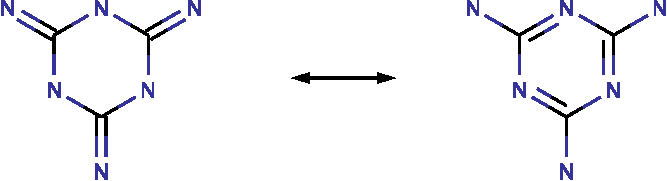
\includegraphics[width=3 true in]{tau-crop}}
        \end{block}
      \end{itemize}
    \item Three different eigensolvers available: native Jacobi
      (slow), GNU scientific library (fast), and Intel's MKL (very
      fast).
  \end{itemize}
\end{frame}


\end{document}
